\documentclass{report} % //TODO find why latex gives errors for report and using textsc!
\usepackage{fancyhdr}
\usepackage{graphicx}
\usepackage{amsmath}
\usepackage{tikz}
\usepackage[margin=1in]{geometry}

\title{UW IND E 250 Notes}
\author{Anthony Le}
 
\newtheorem{exmp}{Example}
\newtheorem{exrc}{Excersize}
\newtheorem{proof}{Proof}
\newtheorem{defn}{Definition}


\begin{document}

\pagestyle{fancy}
\fancyhead{}
\fancyhead[R]{UW IND E 250}
\fancyhead[L]{Anthony Le}

\begin{center}
    \LARGE{\textbf{Chapter 3.1 - Time Value of Money}}
\end{center}

\section*{Time Value of Money}
Focus of Chapter
\begin{enumerate}
    \item Be able to compare the value of money at different points of time
    \begin{enumerate}
         \item Develop a method for reducing a sequence of benefits and costs to a single point in time 
        \item Make our comparisions on that basis
    \end{enumerate}
\end{enumerate}
\section*{Time Value of money}
\begin{enumerate}
    \item Money has a time value since it can earn more money over time (AKA earning power)
    \item Money has a time value where its purchasing power changes over time (AKA inflation)
    \item We measure the time value of money in terms of the market interest rate which reflects both the earning and purchasing power
\end{enumerate}
This isn't only just for money as well! We can associate a time-value to other things - Anything that can be exchanged for money at a margin has a time value to it

\section*{The Interest Rate}
Interest is the cost of money - a cost to the borrower and an earning to the lender.
\newline
Elements of transactions involving interest:
\begin{enumerate}
    \item Principal - amount of money burrowed/invested
    \item Interest rate (i) - measure of price of money, expressed as \%/Period
    \item Interest Period
\end{enumerate}

\section*{Cash Flow Diagram}
From the perspective of the person making the transaction - upward arrows represent "income", and downward arrows represent "payments"
\begin{enumerate}
    \item Important tool in economic analysis
    \item Graphical representation of cash flows drawn on a time scale
\end{enumerate}
\textbf{End of Year Convention} - Any cash flows occuring during the interest period are summed to a single amount and summed to a single number at the end of the interest period
\begin{enumerate}
    \item Think about cash flows "acculiminating" throughout a period - interest rates only taken into account at the end of the period
    \item This is done so banks can make financial calculations easier
    \item Interest periods are typically less than 1 year
\end{enumerate}

\section*{Symbols/Notations}
\begin{enumerate}
    \item [P] - Value/amount of money at present time 
    \item [F] - value/amount of money at future time
    \item [A] - Series of consectutive, equal, end-of-period amount of money
    \item [n/N] - number of interest periods (in years, months, or days)
    \item [i] - interest rate per period (Compounding)
\end{enumerate}

\section*{Simple Interest}
This is interest being charged with respect to the \textbf{base} principal amount. \textbf{This means that the interest stays constant, regardless of the previously accumulated interest.}
    \begin{equation*}
        \begin{aligned}
            F = P + (iP)N
        \end{aligned}
    \end{equation*}

\section*{Compound Interest/Uniform Payment Series}
This is interest being charged with respect to the base principal amount \textbf{AND} previously accumulated interest that hasn't been previously withdrawn.
    \begin{equation*}
        \begin{aligned}
            F = P(1+i)^N
        \end{aligned}
    \end{equation*}

Also to note! All interest rates used in economic analysis are compound interest rates.

\begin{exmp}
    Paying pricipal amount and interest v. interest only
\end{exmp}

\newpage
\begin{center}
    \LARGE{\textbf{Chapter 3.2 - Economic Equivalence}}
\end{center}


\begin{defn}
    \textbf{Economic Equilvalence} \\
    Different sums of money at different times are equal in economic value (As long as interest rates are constant).
\end{defn}

\textbf{Note - This fails to be true whenever the interest rate changes between time periods}

\begin{exmp}
    Find C that makes 2 transactions equivalent at i = 10\%. +\$500 at t = 0, +\$1000 at t = 3
\end{exmp}
For Part A
\begin{equation*}
    \begin{aligned}
        500 + (1+0.1)^2+1000(1+0.1)^{-1}
    \end{aligned}
\end{equation*}

For Part B
\begin{equation*}
    \begin{aligned}
        C + C(1+0.1)^1
    \end{aligned}
\end{equation*}
Set equal to each other and solve

\begin{center} 
    \LARGE{\textbf{Chapter 3.3 - Interest Formulas for Different Types of Cash Flows}}
\end{center}

\section*{F/P Factor (Compound Amount)}
To find F, given i, P, and N:
\begin{equation*}
    \begin{aligned}
        &n = 0:P\\
        &n = 1: F_1 = P(1+i)\\
        &n = 2: F_2=F_1(1+i) = P(1+i)^2\\
        &...\\
        &n = N:F = P(P+i)^N
    \end{aligned}
\end{equation*}

\section*{F/A Factor (Compound Amount Factor)}
To find F, Given i, A, and N:
\begin{equation*}
    \begin{aligned}
        F = A(\frac{(1+i)^n-1}{i})
    \end{aligned}
\end{equation*}
Note - this assumes that there are transactions occuring for every period, including on the last period.

\begin{exmp}
    Given A = \$3000, N = 10 years, and i = 7\% per year, find F
\end{exmp}
\begin{equation*}
    \begin{aligned}
        A = 3000 \quad N = 10 \quad i=7\% \\
        F = A(F/A, i\%, N) \\
        F = 3000(F/A, 7\%, 10) \\
        F = 3000(13.8164) \\
        F = \$41,449.20
    \end{aligned}
\end{equation*}
Alternatively, using the F/A formula to find F:
\begin{equation*}
    \begin{aligned}
        A = 3000 \quad N = 10 \quad i=7\% \\
        F = A(\frac{(1+i)^n-1}{i}) \\
        F = 3000(\frac{(1+0.07)^10-1}{0.07}) \\
        F = 3000(13.8164) \\
        F = \$41,449.20
    \end{aligned}
\end{equation*}

\begin{exmp}
    Derive a formula for doing consectutive deposits starting on year 0, and ending before the final period.
\end{exmp}
To solve this, do the previous formula as normal, (assuming no deposit for the first year) but include a F/P equation for 1 year.

This still simulates the same amount of periods you're depositing money, but now you account for the final period with no deposit.
\begin{equation*}
    \begin{aligned}
        &F = A(F/A, i\%, N)(F/P, i\%, 1) \\
        &F = 3000(F/A, 7\%, 10)(F/P, 7\%, 1) \\
        &F = \$41,449.20(1.07)
    \end{aligned}
\end{equation*}

\begin{exmp}
    Given 3 investment plans - Find the best plan:
    \begin{align*}
        A - A = 2000 \quad N = 10 \quad i=8\% \\
        B - A = 2000 \quad N = 30 \quad i=8\% \\
        C - A = 2000 \quad N = 41 \quad i=8\% \\
    \end{align*}
\end{exmp}
For Plan A, need to first do F/A formula for 1-10 years, then F/P formula for the other 31 years
\begin{equation*}
    \begin{aligned}
        &F = 2000(F/A, 8\%, 10)(F/P, 8\%, 31) \\
        &F = 2000(14.4866)(10.8677) \\
        &F = \$314,870
    \end{aligned}
\end{equation*}
For Plan B, need to do F/A formula for only 31 years
\begin{equation*}
    \begin{aligned}
        &F = 2000(F/A, 8\%, 31) \\
        &F = \$246,691 \\
    \end{aligned}
\end{equation*}
For Plan C, do F/A formula for 41 years
\begin{equation*}
    \begin{aligned}
        &F = 2000(F/A, 8\%, 41) \\
        &F = \$561,562 \\
    \end{aligned}
\end{equation*}

\begin{exmp}
    Comment - Roth IRAs are a way for you to invest money - however, this is based off of your salary bracket. If you exceed a certain cap, you are blocked from investing any more into the plan itself.
\end{exmp}

\section*{A/F Factor (Sinking Fund Factor)}
To find A, Given i, F, and N
\begin{equation*}
    \begin{aligned}
        A = F\frac{i}{(1+i)^n-1}
    \end{aligned}
\end{equation*}
Note - like previous cash flow types, we assume that transactions start on the period N = 1, and continue till the last period N = N

\section*{A/P Factor (Capital Recovery Factor)}
To find A, Given i, P, and N:
\begin{equation*}
    \begin{aligned}
        A = P(\frac{i(1+i)^n}{(1+i)^n-1})
    \end{aligned}
\end{equation*}

\begin{exmp}
    Find the annuity payment given: \\
    P = 250,000 \quad, N = 6, i = 8\%
\end{exmp}
Finding A:
\begin{equation*}
    \begin{aligned}
        A = P(\frac{i(1+i)^n}{(1+i)^n-1}) \\
        A = 250,000(A/P, 8\%, 6) \\
        A = 54,075 \\
    \end{aligned}
\end{equation*}

\begin{exmp}
    Deferred Loan Repayment - Continuing off of previous example: \\
    If the bank allows payments to occur at year 2, find A
\end{exmp}
\begin{enumerate}
    \item Firstly, find (F/P, \%, 1) - Find future value to pay 1 year before annunity payment. This is due to how the bank is continuing to collect interest on the car even though there is a grace period
    \begin{equation*}
        \begin{aligned}
            P = 250,000(F/P, 8\%, 1) \\
            P = 270,000
        \end{aligned}
    \end{equation*}
    \item Afterwards, compute A/P
    \begin{equation*}
        \begin{aligned}
            A = 250,000(F/P, 8\%, 1)(A/P, 8\%, 6) \\
            A = 270,000(A/P, 8\%, 6) \\
            A = 58,401 
        \end{aligned}
    \end{equation*}
\end{enumerate}

\section*{P/A Factor (Present Worth Factor)}
To find P given i, A, and N:
\begin{equation*}
    \begin{aligned}
        P = A\left(\frac{(1+i)^n-1}{i(1+i)^n}\right)
    \end{aligned}
\end{equation*}

To find N given i, A, and P:
Note - will have to use excel's goalseek in order to solve for N. \textbf{Set P to desired P by changing N}

\section*{Arithmetic/Linear Gradient Series}
Linear Gradient Series is a cash flow series that either increases or decreases by a constant amount over n time periods.
\begin{enumerate}
    \item A linear gradient is always comprised of 2 components - the gradient component, and the base annunity component.
\end{enumerate}

\section*{P/G Factor (Present Worth Factor)}  
To find P given i, A, N, and G  
Used only with the gradient section - where you find the present worth of the linear cash flow.
\begin{enumerate}
    \item If G > 0, then you have a increasing gradient series.
    \item If G < 0, then you have a decreasing gradient series.
\end{enumerate}
\begin{equation*}
    \begin{aligned}
        P = G\left[\frac{(1+i)^N - iN -1}{i^2(1+i)^N}\right]
    \end{aligned}
\end{equation*}

\footnote{Note that the first cash flow in a strict linear gradient series is 0.}
\footnote{Also, the tables don't have the future worth of a linear series, so   you'll need to do it by doing P/G first, then finding F/P}

\begin{exmp}
    Given:
    \begin{equation*}
        \begin{aligned}
            A_1 = 1000 \quad G = 250 \quad N = 5 \quad i = 12\%
        \end{aligned}
    \end{equation*}
    Find P:
\end{exmp}
\begin{enumerate}
    \item You know that gradient series are made of the base annunity and the gradient annunity - so 
    \begin{equation*}
        \begin{aligned}
            P = P_1 + P_2
        \end{aligned}
    \end{equation*}
    \item P1 represents the base annunity - so:
    \begin{equation*}
        \begin{aligned}
            P_1 = A_1(P/A,12\%,5) \\
            P_1 = 1000(3.6048)
        \end{aligned}
    \end{equation*}
    \item P2 represents the gradient annunity - so:
    \begin{equation*}
        \begin{aligned}
            P_2 = 250(P/G,12\%,5) \\
            P_2 = 250(6.397)
        \end{aligned}
    \end{equation*}
    \item Adding P1 and P2 together:
    \begin{equation*}
        \begin{aligned}
            P = P_1 + P_2 \\
            P = 1000(3.6048) + 250(6.397) \\
            P = 5204
        \end{aligned}
    \end{equation*}
\end{enumerate}

\section*{A/G Factor (Gradient to Equal Payment Series Factor)}
Finding A given G, i, and N:
\begin{equation*}
    \begin{aligned}
        A = G\left[\frac{(1+i)^N - iN -1}{i(1+i)^N - 1}\right] \\
    \end{aligned}
\end{equation*}
% // TODO - Add A/G Example here!

\newpage
\begin{exmp}
    Linear Gradient Example - \\
    Given: \\
    $A_1$ = 1000 \quad G = 300 \quad N = 6 \quad i = 10\% \\
    Find: \\
    A
\end{exmp}
\begin{enumerate}
    \item Given that we have $A_1$ = 1000, we have our base annunity.
    \item Given that we have G = 300, we have our gradient annunity.
    \item Now that we have everything for the first gradient series - also, since we have our first $A_1$, we don't need to convert to A, however, we do need to convert our gradient annunity to A 
    \begin{equation*}
        \begin{aligned}
            1000 + 300(A/G,10\%,6) = A_{Barb}        
        \end{aligned}
    \end{equation*}
    \item Solving via looking up in tables or plugging into A/G formula:
    \begin{equation*}
        \begin{aligned}
            A_{Barb} = 1667.08
        \end{aligned}
    \end{equation*}
\end{enumerate}

\begin{exmp}
    Given: \quad $A_1$ = 1200 \quad G = -200 \quad N = 5 \quad i = 10\% \\
    Find: \quad F
\end{exmp}
\begin{enumerate}
    \item Firstly, since we don't have a F/P formula, we need to find present from gradient (P/G), when we can find the future value from the present (F/P)
    \item Given that we have the base annuity and can find the future value from the annuity:
    \begin{equation*}
        \begin{aligned}
            1200(F/A,10\%,5)
        \end{aligned}
    \end{equation*}
    \item Finding the present value of the gradient annunity, then converting the present value to future value:
    \begin{equation*}
        \begin{aligned}
           &= -200(P/G,10\%,5)(F/P,10\%,5)\\
           &= x %//TODO - complete example by adding values and steps!
        \end{aligned}
    \end{equation*}
\end{enumerate}

\begin{exmp}
    Given: \quad $A_1$ = 15000 \quad G = -1000 \quad N = 12 \quad i = 8\% \\
    Find: \quad A (Equal Payment Series)
\end{exmp}
\begin{enumerate}
    \item Converting Gradient Series to Equal Payment Series:
    \begin{equation*}
        \begin{aligned}
            -1000(A/G,8\%,12)
        \end{aligned}
    \end{equation*}
    \item Setting up Equation and solving - have first equal payment series done already
    \begin{equation*}
        \begin{aligned}
             &= 15000 -1000(A/G,8\%,12) \\
             &= x %//TODO - Add in final value for example!
        \end{aligned}
    \end{equation*}
\end{enumerate}

\begin{exmp}
    Given: \quad $A_1$ = 10000 \quad G = 3000 \quad N = 5 \quad i = 8\% \\
    Find: \quad F %//TODO - Unsure whether this is what you're finding
\end{exmp}
%//TODO - Add in example and steps!

\newpage
\section*{Geometric Series}
Similar to linear gradient series, but it is based off of a \textbf{percentage} rather than a fixed amount/number

\begin{equation*}
    \begin{aligned}
        &P = \frac{A_1}{i-g}\left[1-\left(\frac{1+g}{1+i}\right) ^N \right] &\text{if i is not equal to g} \\
        &P = \frac{NA_1}{1+i} &\text{if i equals g}
    \end{aligned}
\end{equation*}
\footnote{These formulas are dependent on whether i and g are equal to each other}

\begin{exmp}
    Given: \quad F = 100000 \quad g = 6\% \quad N = 20 \quad i = 8\% \\
    Find: \quad $A_1$
\end{exmp}

\begin{enumerate}
    %\item Note that to find $A_1$ given the future value, you'll need to 
    \item You'd solve the problem by converting the base annuity value to present value, then convert present value to future value.
    \item Setting up equation:
    \begin{equation*}
        \begin{aligned}
            F = A_1(P/A_1,6\%,8\%,20)(F/P,8\%,20)
        \end{aligned}
    \end{equation*}
\end{enumerate}
%//TODO - Add in steps for example and plug in numbers and solve! 
\begin{center}
    \LARGE{\textbf{Chapter 3.3 - Development of Formulas for Equivalence Calculations}}
\end{center}

\section*{Combining Factors}
Most estimated cash flow series don't fit the factors and equations exactly. In these cases you'll be combining the engineering economy factors in order to determine either equilivalent present worth (P), future worth (F), or annual worth (A)

\section*{Shifted Uniform Series}
This is a series of which whose present worth point in time is NOT t = 0, but is instead shifted to the left or to the right.

\begin{exmp}
    Reference Lecture 4 Example 1: \\
\end{exmp}
To have everything balance so i = 12\% 
\begin{enumerate}
    \item Not exactly describing the process, but the example goes through and continiously uses P/F to find the present worth of various items, like the annual payments and regular payments - use these to convert to present value - something like this %/TODO - add in examples and complete!
    \item Overall - set up equations for cash flow in and out - setting these equal to each other to find x
\end{enumerate}

\begin{exmp}
    Referecnce Lecture 4 Example - Cash Flows with missing payments
\end{exmp}
\begin{enumerate}
    \item treat problem as equal payments, but subtract one 
\end{enumerate}

\footnote{Note - check out the github page for the week 2 overview if you're confused on the concepts taught during class! This includes graphics and explainations to help explain said concepts.}

\section*{What have we learned so far?}
\begin{enumerate}
    \item Time value of money
    \item Economic equilvalence
    \item how to look up table
    \item Uniform payment series, uneven series, and gradient series.
\end{enumerate}

\begin{exmp}
    Reference Lecture 4 - Practice example for quiz 1 
\end{exmp}
Find the value of x so the two cash flow shown in the diagram are equilivalent for an interest rate of 8\%

(Teacher solution) Move all transactions over to the future:
\begin{equation*}
    \begin{aligned}
        200(F/A,8\%,5) - 50(F/A,8\%,1) 
    \end{aligned}
\end{equation*}
For the second cashflow diagram - you do the same process of moving all transactions to the future - do a recurring F/A for 5 years for x with subtracting 200+x for 1 year and 2 years respectively:
\begin{equation*}
    \begin{aligned}
        &X(P/A,8\%,5) - [(200+X)(P/F,8\%,3)+ (200+X)(P/F,8\%,4)] \quad \text{Alternatively,} \\
        &(X+200)(F/A,8\%,2)(F/P,8\%,2)(F/P,\%,1)
    \end{aligned}
\end{equation*}
Set up problem by doing P/A for a constant value for 5 years:
\begin{equation*}
    \begin{aligned}
        200(P/A,8\%,5) - 50(P/A,8\%,1)
    \end{aligned}
\end{equation*}

\begin{center}
    \LARGE{\textbf{Chapter 4 - Understanding Money and its management}}
\end{center}
\section*{Ch 4 - What to expect}
\begin{enumerate}
    \item Know the different between the nominal interest rate and effective interest rate
    \item The procedure for computing the effective interest rate, based on a payment period
    \item How commercial loans and mortgages are structured.
\end{enumerate}

\section*{Terminology}
\begin{enumerate}
    \item Ch.3
    \begin{enumerate}
        \item If not indicated, interest earned annually, including inflation
    \end{enumerate}
\end{enumerate}

\section*{4.1 - Nominal and Effective Interest Rates}
\begin{defn}
    \textbf{Nominal Interest Rate} \\
    Interest Rate quoted based on an annual period.
\end{defn}

\begin{defn}
    \textbf{Effective Interest Rate} \\
    Actual interest earned/paid in a year or some other time period. \\
    Note - companies/etc are required by law to give you the true effective interest rate.
\end{defn}

Ex: Breaking down interest rate - 18\% compounded monthly:
\begin{enumerate}
    \item What does it really mean?
    \begin{enumerate}
        \item Interest rate per month (i) = 18\%/12 = 1.5\%
        \item Number of interest periods per year = 12
    \end{enumerate}
    \item In other words:
    \begin{enumerate}
        \item Bank will charge 1.5\% interest every month on unpaid balance, or
        \item You'll earn 1.5\% interest each month on your remaining balance
    \end{enumerate}
\end{enumerate}

\begin{exmp}
    If you interest \$1 for 1 year at 18\% interest compounded monthly, how much would you earn?
\end{exmp}
%//TODO - add in example from slides!
\textbf{Formula:} 
\begin{equation*}
    \begin{aligned}
        i_a = (1+ r/M)^M - 1
    \end{aligned}
\end{equation*}
Where: \\ %//TODO format this better, center me!
r = nominal interest rate per year \\
$i_a$ = effective annual interest rate \\
M = number of interest periods per year \\

\noindent
More advanced verion:
\begin{equation*}
    \begin{aligned}
        i_a = (1+ r/CK)^C - 1
    \end{aligned}
\end{equation*}
Where: \\ %//TODO format this better, center me!
r = nominal interest rate per year \\
C = number of interest periods per payment period \\
K = number of payment periods per year
CK = M = number of interest periods per year \\

For example, of 18\% compounded monthly:
\begin{equation*}
    \begin{aligned}
        i_a &= (1 + 0.18/12)^12 - 1 \\
            &= 19.56\%
    \end{aligned}
\end{equation*}

\begin{exmp}
    Lecture 4 Ch3Ch4 Example - find effective interest rate for 9\% compounded quarterly:
\end{exmp}
\begin{equation*}
    \begin{aligned}
        &i = 9\% \quad M = 4 \\
        &r = i/M = 9/4 = 2.25\% \\
        &i_a = \left(1 + \frac{0.225}{4}\right)^4 - 1 \\
        &i_a = 9.31\%
    \end{aligned}
\end{equation*}
And for P = \$10,000:
\begin{equation*}
    \begin{aligned}
        &F = 10000(F/P,9.31\%,1), \quad \text{OR} \\
        &F = 10000(F/P,2.25\%,4) \\
    \end{aligned}
\end{equation*}
The second approach does the same thing in the end, but you're using periods of \textbf{quarters}, not YEARS

\section*{Annual Percentage Rate (APR)}
\begin{defn}
    \textbf{APR} \\
    in the US, APR is expressed as the periodic interest rate times
    the number of compounding periods in a year (the nominal
    interest rate!)    
\end{defn}

\section*{Why do we need effective interest rate per payment period?}
We need to do this to account for cases where payment and compounding periods differ from each other and transform so that all different cash flow types conform to the same unit of time.

Generalized Version of Compound Interest Formula:
\begin{equation*}
    \begin{aligned}
        i_a = (1+ r/CK)^C - 1
    \end{aligned}
\end{equation*}
Where: \\ %//TODO format this better, center me!
r = nominal interest rate per year \\
C = number of interest periods per payment period \\
K = number of payment periods per year \\
CK = M = number of interest periods per year \\

\begin{exmp}
    Find Effective interest rate per payment period: \\
    9\% compounded monthly \quad Payments quarterly:
\end{exmp}
\begin{enumerate}
    \item Know that payment periods are quarterly, so
    \begin{equation*}
        \begin{aligned}
            K = 4
        \end{aligned}
    \end{equation*}
    \item Know annual interest, so 
    \begin{equation*}
        \begin{aligned}
            &r = 9\% 
        \end{aligned}
    \end{equation*}
    \item Know that interest compounds monthly, and there are 3 months per quarter:
    \begin{equation*}
        \begin{aligned}
            C = 3
        \end{aligned}
    \end{equation*}
    \item Plugging into compound interest equation:
    \begin{equation*}
        \begin{aligned}
            i_a &= (1 + r/CK)^C - 1 \\
                &= (1 + 9\%/(3*4))^3 - 1 \\
            i_a &= ???? %//TODO - plug in and calculate effective interest rate!
        \end{aligned}
    \end{equation*}
\end{enumerate}

\begin{exmp}
    Find Effective interest rate per payment period with continious compounding: \\
    $C \rightarrow \infty$
\end{exmp}
Writing out formula for continious compounding:
\begin{equation*}
    \begin{aligned}
        &i = \lim_{C \rightarrow \infty}(1+r/CK)^C - 1 \\
        &i = e^r - 1
    \end{aligned}
\end{equation*}

\section*{Single-Payment transactions with continious compounding - future and present worth}

Finding Future Worth given Present Compounded Continiously:\footnote{can also use the formulas used in class with continious compounding interest by doing $i_a = e^r-1$}
\begin{equation*}
    \begin{aligned}
        F &= P(1+i)^N \\
          &= Pe^{rN}
    \end{aligned}
\end{equation*}

Finding Present Worth given Future Compounded Continiously:
\begin{equation*}
    \begin{aligned}
        F &= P(1+i)^N \\
          &= Pe^{rN}
    \end{aligned}
\end{equation*}

\section*{Equilivalence Calculations using Effective Interest Rates}
\begin{enumerate}
    \item Identify the payment period (annual,quarterly,etc)
    \item Identify interest period
    \item Find the effective interest rate that covers the payment periods
\end{enumerate}

\subsection*{Case 1: When Payment Period = Compounding Period}
\begin{enumerate}
    \item Identify the number of compounding periods per year
    \item Compoute the effective interest rate per year
    \item Compute the payment periods per year
\end{enumerate}

\begin{exmp}
    Calculating auto loan payments
\end{exmp}
\begin{center}
    \begin{enumerate}
        \item Price = 20,870
        \item Discounts = 2,443
        \item Net Sale Price = 18,427
        \item Down Payment = 3,427
        \item Dealer Interest Rate = 6.25\%, compounded monthly
        \item Length of financing  = 72 months = 6 years
    \end{enumerate}    
\end{center}
After taking out discounts and down payment - you're left with 15000. 
\newline
\begin{enumerate}
    \item Finding i:
    \begin{equation*}
        \begin{aligned}
            i = 6.25/12 = 0.520833\%
        \end{aligned}
    \end{equation*}
    \item Finding monthly payment:
    \begin{equation*}
        \begin{aligned}
            &A = 15,000(A/P,0.5208\%,72) \\
            &A = 250.37
        \end{aligned}
    \end{equation*}
\end{enumerate}

\begin{exmp}
    Compute how much money you would have if you paid 3.00 every day for 30 years, assuming you earn 5\% interest (nominal interest rate per year).
\end{exmp}
\begin{enumerate}
    \item Converting into effective interest rate:
    \begin{equation*}
        \begin{aligned}
            i = 5\%/365 = 0.0137\%/day
        \end{aligned}
    \end{equation*}
    \item Getting future worth given annuity payment:
    \begin{equation*}
        \begin{aligned}
            F = 3(F/A, 0.0137\%, 30*365) \\
            F = 76,246
        \end{aligned}
    \end{equation*}
\end{enumerate}

\subsection*{Case 2: When payment periods differ from compounding periods}
\begin{enumerate}
    \item Identify M, K, and C
    \item Compute the \textbf{effective interest rate per payment period}
    \begin{enumerate}
        \item For discrete compounding:
        %//TODO - include discrete compounding formula here!
        \item For continious compounding:
        %//TODO - include continious compounding formula here!
    \end{enumerate}
    \item FInd the total number of payment periods
    \item Use i and N in the appropiate equilivalence formula
\end{enumerate}

\begin{exmp}
    Compounding occurs more frequently than payments are made (Discrete Case)
\end{exmp}
\begin{center}
    A = 1,500 per quarter \\
    N = 2 years \\ 
    r = 6\% compounded monthly \\
    Find F
\end{center}
\begin{enumerate}
    \item Converting interest rate to monthly:
    \begin{equation*}
        \begin{aligned}
            i = 6\%/12 = 0.5\%/Month
        \end{aligned}
    \end{equation*}
    \item Converting interest rate to quarterly:\footnote{Note, the 3 represents the number of interest periods in a single payment period.}
    \begin{equation*}
        \begin{aligned}
            (1 + 0.5\%)^3 - 1 = 1.5075\%/Quarter
        \end{aligned}
    \end{equation*}
    \item Getting future worth from annuity:
    \begin{equation*}
        \begin{aligned}
            F = 1500(F/A,1.5075\%,8)
        \end{aligned}
    \end{equation*} 
\end{enumerate}

\begin{exmp}
    Compounding occurs less frequently than payments are made (Discrete Case)
\end{exmp}
\begin{center}
    A = 500 per monthly \\
    N = 10 years \\ 
    r = 10\% compounded quarterly \\
    Find F
\end{center}
\begin{enumerate}
    \item Converting interest rate to be per quarter
    \begin{equation*}
        \begin{aligned}
            i = 10\%/4 = 2.25\%/Quarter
        \end{aligned}
    \end{equation*}
    \item Splitting interest payments to be equal across each payment period\footnote{I'm not quite sure why we would do it this way}
    \item Alternatively, describing the problem using M, K, and C
    \begin{center}
        M = Compounding Periods/Year = 4 \\
        K = Payment Periods/Year = 12 \\
        C = Interest Periods/Payment Periods = 4/12 = 1/3 \\
    \end{center}
    \item Getting monthly interest rate from C
    \begin{equation*}
        \begin{aligned}
            i = (1+i)^C \\
            i = (1+2.5\%)^{1/3} \\
            i = 0.26
        \end{aligned}
    \end{equation*}
    \item Getting Future Worth given annuity: \\
    \begin{equation*}
        \begin{aligned}
            F = (F/A, )
        \end{aligned}
    \end{equation*}
\end{enumerate}

\section*{Chapter 4.5 Debt Management}
\begin{defn}
    \textbf{Amortized Loan} \\
    Loan is repaid in equal periodic amounts. \\
    \begin{equation*}
        \begin{aligned}
            &B_n = \text{Remaining balance at the end of period n, with} B_0 = P\\
            &I_n = \text{Interest Period in }\\
            &P_n 
        \end{aligned}
    \end{equation*}
\end{defn}

\begin{exmp}
    Example 4.13 - Loan Balance, principal and interest remaining - balance period  
\end{exmp}
\begin{center}
    Given: \\
    P = 5000, 12\% APR, N = 24 months \\
    Find: Loan balance, loan 
\end{center} %//TODO - Include example 4.13 in notes! I'm sorry but i haven't had the time to work on my notes and add in the xamples from the class.
\section*{Calculating the remaining loan balance after making nth payment}
\subsection*{Remaining-Balance Method}
Alternatively, we can derive $B_n$\footnote{$B_n$ is the remaining balance, $P_n$ the principal payment (Or how much of your annunity payment goes to your loan)} by computing the equivalent payments remaining after the nth payment. Thus, the balance with N-n payments remaining is:
\begin{equation*}
    \begin{aligned}
        B_n = A(P/A,i,N-n)
    \end{aligned}
\end{equation*}
And the interest payment during period during n is:
\begin{equation*}
    \begin{aligned}
        I_n = (B_{n-1}i) = A(P/A,i,N-n+1)i 
    \end{aligned}
\end{equation*}
Where $A(P/A,i,N-n+1)i$ is the balance remaining at the end of period n-1 and:
\begin{equation*}
    \begin{aligned}
        P_n &= A - I_n = A - A(P/A,i,N-n+1)i\\
            &=A(1-(P/A,i,N-n+1)i)
    \end{aligned}
\end{equation*} 
Knowing the interest factor relationship (P/F,i,n) = 1-(P/A,i,n)i from table 3.6, we obtain:
\begin{equation*}
    \begin{aligned}
        P_n = A(P/F,i,N-n+1)
    \end{aligned}
\end{equation*} 

\begin{exmp}
    Example 4.15 - Financing your vehicle
\end{exmp}
\begin{center}
    Three financing options - debt, cash or lease \\
    Payment Period - Monthly \\
    Interest Period - Monthly \\
    Cost = \$32,508
\end{center}
\begin{enumerate}
    \item Debt Financing (Find Monthly Payment) 
    \begin{equation*}
        \begin{aligned}
            A &= (32508-4500)(A/P,\frac{5.65}{12},42) \\
            A &= \$736.53
        \end{aligned}
    \end{equation*}
    Where the Car costs \$32,508, down payment of \$4,500, APR of 5.65\%
    \item Cash Financing
    \begin{equation*}
        \begin{aligned}
            P = 4500 + 736.53(P/A,\frac{4.5\%}{12},42) - \$17,817(P/A,\frac{4.5\%}{12},42)\\
            P = \$17,847
        \end{aligned}
    \end{equation*}
    \begin{equation*}
        \begin{aligned}
            P = 31020 - 17847(P/F,4.5\%,42) \\
            P = \$15,845
        \end{aligned}
    \end{equation*}
\end{enumerate}

\section*{Home Morgage}
Morgages are loans for buying property. These have mothly payments and compounding.
Types of Home Morgages:
\begin{enumerate}
    \item Fully Amortizing Mortage:
    \begin{enumerate}
        \item Fixed-rate mortgage
        \item Adjustable-rate mortgage
        \item Hybrid mortgage
    \end{enumerate}
    \item Interest-based mortgage
\end{enumerate}

The cost of mortgage:
\begin{enumerate}
    \item Loan amount
    \item Loan term
    \item Payment frequency
    \item Points (prepaid interest)\footnote{this is where you pay a fee to lower the interest rate by a point (not a percentage! I think it's like 1/4 of a percent - this rate is about \$5000 per point)}
\end{enumerate}

\begin{exmp}
    Example 4.16 - Interst-only vs. Fully Amortized mortgage
\end{exmp}
\begin{center}
    Given: P = 200000, 6.6\% compounded monthly, N = 30
\end{center}
\begin{enumerate}
    \item Fully Amortized payment:
    \begin{equation*}
        \begin{aligned}
            A = 200,000(A/P,\frac{6.6}{12},360) = 1277.32
        \end{aligned}
    \end{equation*}
    \item Five-year interest only option:
    \begin{equation*}
        \begin{aligned}
            A = 200,000(0.0055) = 1100
        \end{aligned}
    \end{equation*}
\end{enumerate}

\begin{exmp}
    Example 4.18 - Hybrid adjustable mortgage plan
\end{exmp}
\begin{center}
    Given: Loan = 100,000, N = 30
\end{center}

To find annunity payments for years 1-5, do A/P for your inital loan with the term length
Afterwards, if you want to find the remaining balance for the other years, take $B-n$ = A(P/A,i,term length - previous term length) - AKA for the first 5 years, the previous term length would be 60 months

\section*{Section 4.6A - Investment Basics}
Right investment is a balance of liquidity, safety, and return.
\begin{enumerate}
    \item Liquidity - should avoid being TOO liquid as you have to take into account inflation, money LOSES value
    \item Safety
    \item Return
\end{enumerate}

\subsection*{Components of expected return}
\begin{enumerate}
    \item Real return
    \item inflation
    \item risk premium (corresponds to how much "risk" you have AKA how likely you are to lose or gain money)
    \item total expected return
\end{enumerate}

\section*{Midterm Exam}
\begin{enumerate}
    \item Must show work! Partial credit
    \item 6 problems to do
    \item Have entire class time to do work
    \item Factor tables and percentages are provided
    \item For problems asking for factored notation, write out setup, but don't solve!
    \item Only 1 bond problem - multiple choice
\end{enumerate}

\subsection*{B. Investment Strategies}
\begin{enumerate}
    \item Trade-off between risk and reward:
    \begin{enumerate}
        \item Cash - least risky with lowest returns
        \item Debt - moderately risky with moderate returns
        \item Stocks/Equities - most risky bu offers greatest payoff
    \end{enumerate}
    \item Note- Broader diversification reduces risk - by combining assets with different patterns of return, it's possible to achieve higher rate of return without increasing risk
    \item Portfilios for long term requires equities to offset inflation, while short time frames require debt or cash investments to reduce volatility
    \item\textbf{Dollar-Cost Averaging} - buying a fixed dollar amount of a particular investment on a regular schedule, regardless of a share price
\end{enumerate}

\subsection*{C. Investing in stocks}
Investing in stocks and bonds is one of the most common investment activities among American investors

\section*{Stock Index}
Measures the value of a section of the stock market - AKA a way to measure the performance of a section of the stock market, examples such as:
\begin{enumerate}
    \item DOW
    \item Wilshire 5000
    \item NASDAQ Composite
    \item Russell 2000
    \item S\&P 500 - based on market capitalizations of the top 500 companies
\end{enumerate}

\section*{What ae bonds?}
As a business grows, if the company doesn't generate enouygh cash internally to pay for its liabilities (ex supplies, equipment required to grow), there are methods to generate money:
\begin{enumerate}
    \item Stocks
    \item Bonds
\end{enumerate}

\subsection*{D. Investing in Bonds}
Bonds are loans that investors make to corporations and goverments.
\begin{enumerate}
    \item Face (par) value - principal amount (typically 1-10 thousand dollars)
    \item Coupon rate - Nominal interest rate quoted on par value
    \item Maturity - the value of the loan
\end{enumerate}

\subsection*{Types of bonds}
\begin{enumerate}
    \item Corporate Bonds
    \item Treasury Bonds
    \item Municipal Bonds - typically nonprofit bonds (ex public services)
    \item Junk Bonds - more risky bonds, typically with higher coupon rate in order to incentivise people to raise money
\end{enumerate}

\subsection*{Mutual Fund}
A pool of funds collected from many investors form the purpose of investing in stocks, bonds, money market instruments (ex: a college fund) with a specified rate of return.
\begin{enumerate}
    \item Plans will move money around from bonds to stocks etc.
\end{enumerate}

%//TODO - For caitlin, we finished lecture 6 and are moving into lecture 7!

\subsection*{Bond Price Notation used in financial markets}
\begin{enumerate}
    \item Bonds - 1 point = \$10, 1/8
    \item Treasury - 1 point = \$10, 1/32 
\end{enumerate}

\subsection*{How do prices and yields work?}
\begin{enumerate}
    \item Yield to Maturity - Actual interest earned from bond over holding period (use to estabilish econ. equilbalnce)
    \item Current Yield - Annual interest earned as a percentage of the current market price
\end{enumerate}

\begin{exmp}
    4.20 - Yield to Maturity and Current Yield
\end{exmp}
Givens:
\begin{enumerate}
    \item Face Value = 1000
    \item Purchase Price = 996.25
    \item Coupon Rate = 9.625\% or 4.8125\% semi-annually\footnote{Coupon payments  = interest rate per payment period * face value}
\end{enumerate}
Find: 
\begin{enumerate}
    \item Yield to maturity - AKA interest "i" earned over life of the bond\footnote{You won't exactly have to do this process on the exam, and you'll have the tables to work with}
    \begin{equation*}
        \begin{aligned}
            &996.25 =(4.8125\% *  1000) (P/A,i,20) + 1000(P/F,i,20)\\
            &996.25 =(48.13)(P/A,i,20) + 1000(P/F,i,20) \quad \text{Solving for i via P/A and P/F equations}\\ 
            &i = 4.84\% \quad \text{semiannually} \\ %//TODO - How do you manage to solve for i in the P/A and P/F equations? this seems very tedious to work with the equations
            &i = 4.84\% * 2 = 9.68\% \quad \text{nominal, annually} \\
            &i_a = (1+4.84\%)^2-1 = 9.914\% \quad \text{effective annual}
        \end{aligned}
    \end{equation*}
    \item Current Yield
    \begin{equation*}
        \begin{aligned}
            \frac{\$48.13}{\$996.25} = 4.83\% \quad \text{semiannually} \\
            i_a = (1+4.83\%)^2-1 = 9.9\% 
        \end{aligned}
    \end{equation*}
\end{enumerate}

\begin{exmp}
    Bond Value over Time
\end{exmp}
Continuing from previous example: \\
Givens:
\begin{enumerate}
    \item Face Value = 1000
    \item Purchase Price = 996.25
    \item Coupon Rate = 9.625\% or 4.8125\% semi-annually\footnote{Coupon payments  = interest rate per payment period * face value}
\end{enumerate}
\begin{enumerate}
    \item Current Value of Bond 1 Year Later:\footnote{Since we are finding the value of the bond 1 year later, we take off 2 payment periods, making the periods left 20-2 = 18 periods}
    \begin{equation*}
        \begin{aligned}
            &48.13(P/A,4.84\%,18) + 1000(P/F,4.84\%,18) \\
            &= 996.80 
        \end{aligned}
    \end{equation*}
    \item Current Value of Bond 1 Year Later, at a interest rate of 9\%
    \begin{equation*}
        \begin{aligned}
            &48.13(P/A,4.5\%,18) + 1000(P/F,4.5\%,18) \\
            &=1038.06 \quad \text{This is called the max price bid}
        \end{aligned}
    \end{equation*}
    In this case, the bond would sell at a premium over its par value - Generally, 
    \begin{enumerate}
        \item As the interest rate decreases ... ??? (Something relating to maturity and coupon payments)
        \item As the interest rate increases ... ??? (Something relating to maturity and coupon payments)
    \end{enumerate}
\end{enumerate}
%//TODO - Send Annika your notes for the midterm!
\section*{Practice Exam Workthrough}
\subsection*{Problem 2} 
To solve the problem, evaluate the present value of options A and B 
Put in equilvalent transactions!
\begin{enumerate}
    \item Option A - purchase the car at \$26,200 with 2 year loan at 3\% APR compounded monthly: 
    \begin{equation*}
        \begin{aligned}
            A = 26200(A/P,3\%/12,24) = 1126.60
            P = 1126.60(P/A,)
        \end{aligned}
    \end{equation*}
    \item Option B - purchase the car \$24,000 with 2 year "loan" at 6\% APR compounded monthly:\footnote{pretending the mutual fund is a loan}
    \begin{equation*}
        \begin{aligned}
            A = 24000(A/P,6\%/12,24) = 1063.20
        \end{aligned}
    \end{equation*}
\end{enumerate}

\section*{Chapter 11}
\section*{11.1 Meaning and Measure of Inflation}
\begin{enumerate}
    \item Inflation: Same dollars buys less goods over time (loss in the purchasing power over time)
    \item Deflation: Price decreases over time (gains in purchasing power)
    \item Consumer Price Index (CPI): Measures the general increase in prices of consumer products by comparing the cost of typical market basket between periods
    \begin{enumerate}
        \item Masket basket of goods and services (8 major groups)
        \begin{enumerate}
            \item Food/alcoholic beverages
            \item Housing 
            \item Apparel
            \item Transportation
            \item Medical care
            \item Transportation
            \item Entertainment
            \item Personal care
            \item Others
        \end{enumerate}
        \item Base period: A point in the past for comparision
    \end{enumerate}
\end{enumerate}

\section*{Average Inflation Rate}
Average Inflation Rate (f) - geometric average over a several-year period

\section*{General Inflation Rate}
General Inflation Rate $\bar{f}$ - the average inflation rate based on the CPI for all items in the market basket

\section*{11.2 Actual versus Constant Dollars}
\begin{enumerate}
    \item Actual dollars: Out of pocket dollars paid at the time of purchasing goods and services; determined by applying an inflation rate to base-year dollars
    \item Constant (real) dollars: represent dollars expressed in terms of the purchasing power of the base-year; used to adjust for the effects of inflation
\end{enumerate}
We use this to compare the relative performance of things, takig into the account of inflation

\section*{Conversion from constant to actual dollars}
\begin{exmp}
    Converting a 1000 cash floor at year 3 estimated in constant dollars of year 0 to its equivalent actual dollars at tht esame period assuming an 8\% inflation rate
\end{exmp}
\begin{equation*}
    \begin{aligned}
        A-n = A_n' (1+f)^{-n} \leftrightarrow
    \end{aligned}
\end{equation*}

\section*{11.2 Equivalence Calculation under Inflation}
\begin{enumerate}
    \item Market interest rate (i): Accounts for both earning and urchasing power; quoted by financial instutitions
    \item Inflation-free interest rate (i'): an estimate ofthe true earning power (AKA real interest rate)
    \item Calculating cash flow equivalence we convert all cash flow into one type through either Constant-dollar analysis or Actual-dollar analysis
\end{enumerate}

\section*{Adjusted-Discount Method}
Performing deflation and discounting in 1 step:
\begin{equation*}
    \begin{aligned}
        P_n &= \frac{\frac{A_n}{(1+\bar{f})^n}}{(1+i')^n} \quad P_n = \frac{A-n}{(1+i)^n}\\
        &= \frac{A_n}{(1+\bar{f})^n(1+i')^n} \quad (1+i) = (1+\bar{f})(1+i') \\
        &= \frac{A_n}{[(1+\bar{f})(1+i')]^n} \quad i = i' + \bar{f} + i'\bar{f}
    \end{aligned}
\end{equation*}

%//TODO - do notes from Monday 4/24/23 CH11CH5 Notes!
\section*{Chapter 5 - Present Worth Analysis}
\subsection*{Alternatives}
\begin{enumerate}
    \item Creation of \emph{"Alternatives"}:
        \begin{enumerate}
            \item If there are no alternatives to consider then there is really no problem to solve!
        \end{enumerate}
    \item Given a set of \emph{"feasible"} alternatives, engineering economy attempts to identify the \emph{"best"} economic approach to a given problem
        \begin{enumerate}
            \item Feasible means "viable" or "doable"
            \item Part of Engineering Econ is the \emph{selection} and execution of the best alternative from among a set of feasible alternatives
        \end{enumerate}
\end{enumerate}
\section*{Section 5.1 - Three Types of Categories}
Formulating Alternatives:
\begin{enumerate}
    \item The Single Project
    \item Mutually Exclusive Set
    \item Independent Project Set
\end{enumerate}

\subsection*{The Single Project}
\begin{enumerate}
    \item The unconstrained project selection problem
    \item No comparision to competing projects
    \item Acceptance or rejection is based on comparision with the firm's opportunity cost (always present)
    \item Two Alternatives
        \begin{enumerate}
            \item Do nothing (reject the project)
            \item Accept the project
        \end{enumerate}
    \item Do Nothing
        \begin{enumerate}
            \item Involve the alternative use of the firm's funds that could be invested in the project!
            \item Maintaining the status quo may not be an option
        \end{enumerate}
\end{enumerate}
\subsection*{Mutually Exclusive Set}
\begin{enumerate}
    \item Mutually Exclusive Set (Only \emph{one} of the feasible projects can be completed)
    \item It is the set is comprised of "do-able" feasible alternatives
    \item Alternatives compete with each other! 
    \item Think buying vs leasing a car
\end{enumerate}
\subsection*{Independent Project Set}
\begin{enumerate}
    \item Independent Set
        \begin{enumerate}
            \item More than 1 can be selected
            \item Deal with budget limitations
            \item Project dependencies and relationships
            \item Example - improve public infrastructure by building roads, public library, schools, etc.
        \end{enumerate}
    \item More involved analysis
        \begin{enumerate}
            \item Often formulated as a 0-1 linear programming model
            \item With constraints and an objective function
        \end{enumerate}
\end{enumerate}
\subsection*{Payback Period Analysis}
\begin{enumerate}
    \item Screens project based on the payback period
    \item Technique: estimates the time $n_p$ to recover the \emph{inital investment} in a project, either with or without investment earned
    \item Two Forms:
        \begin{enumerate}
            \item With no interest $\rightarrow i = 0\%$ (no-return/traditional payback ) 
        \end{enumerate}
\end{enumerate}
%//TODO - Continute off of CH11Ch5 Slides Page 32 of 50!



%//TODO - Do notes from slides 1-14 CH5 Notes!
\section*{Section 5.5: Comparing Mutually Exclusive Alternatives}
\subsection*{Review: Net Present Worth}
\begin{enumerate}
    \item Net Present Worth (NPW): The difference between the present worth of all cash inflows and outflows.
    \item Decision Rules for Single Prject Evaluation: Accept the project if the NPW is \textbf{positive}.
    \item Decision Rule for Comparing Multiple Alternatives: Select the alternative with the largest net present worth.
    \item Minimum attractive rate of return (MARR): The required rate of return, or the interest rate firm can always invest the money in its investment pool.
\end{enumerate}

\section*{Comparing Mutually Exclusive Projects - Basic Terminologies}
So far, you've only considered projects with equal lifetimes:
\begin{enumerate}
    \item Mutually Exclusive Projects: One of them fufills the same need
    \begin{enumerate}
        \item Selecting one = excluding other options
    \end{enumerate}
    \item Alternative and Projects are going to be used interchangeably
    \begin{enumerate}
        \item Revenue Projects
        \item Service Projects
    \end{enumerate}
\end{enumerate}

\section*{Revenue Vs Service Projects}

Revenue Projects:
\begin{enumerate}
    \item Revenue and cost streams vary with choice of alternatives
    \item Maximize net income = pick higher net present worth
\end{enumerate}

Service Projects:
\begin{enumerate}
    \item Fixed/Constant revenues for all alternatives
    \item Minimize expenditures = pick the lower present-value production cost AKA chose the alternative that costs you the least amount of money
\end{enumerate}

\section*{Comparing Mutually Exclusive Projects}
\begin{enumerate}
    \item Principle - Projects must be compared over an equal time span
    \item Rule of Thumb - If the required service period is given, the analysis period should be the same as the required service period.
\end{enumerate}

\section*{Case 1: Revenue Projects with Equal Lives}
Where analysis period equals project lives \\
What to do:
\begin{enumerate}
    \item Compute NPW for each projec over its life and select the project with the largest NPW
\end{enumerate}
What if alternate lives are different?
\section*{Present Worth Analusis of Different Life Alternatives}
\begin{enumerate}
    \item For Alternatives with un-equal lives the rule is:
    \item PW of alternatives must be compared over the same number of years
\end{enumerate}
This approach is called the "equal service" requirement.
Approach:
\begin{enumerate}
    \item Analysis Period: assume a planning horizon and evaluate the alternatives over this number of years (Cases 2,3,4)
    \item LCM: Evaluate the alternatives over the \textbf{lowest common multiple} of lives (ex project lives of 4 and 6, use n = 12 and assume re-investment at same properties)
\end{enumerate}

\begin{exmp}
    Remove radioactive materials using a bulldozer. 2 Models A and B - where the job can be completed for 2 years.
    \begin{enumerate}
        \item MARR = 15\%
        \item Model A - operate 3 years
        \item Model B - operate 6 years
    \end{enumerate}
\end{exmp}
Find:
\begin{enumerate}
    \item Estimate the salvage value at the end of the required service period
    \item Find the NPW at the end of the service period
\end{enumerate}
For this service project, you'll be selecting off of the lowest NPW and be using a analysis period of 3 years since 3 is the lowest common denominator between 3 and 6.
Finding PNW
\begin{enumerate}
    \item Finding for model A:
        \begin{equation*}
            \begin{aligned}
                PW(15\%) &= -300 + -80(P/A,15\%,2) \\
                    &= -362
            \end{aligned}
        \end{equation*}
    \item Finding for model B:
        \begin{equation*}
            \begin{aligned}
                PW(15\%) &= -480 + -45(P/A,15\%,2) \\
                &= -364
            \end{aligned}
        \end{equation*}
    \item Select model A as it has a lower NPW.
\end{enumerate}

\section*{Case 3: Project Lives Shorter Than Analysis Period}
To solve this, you'll need to come up with replacement projects that match the required service period. IRL, you'll have to do research on what to select for the replacement project - ie renting/leasing an asset

\section*{Case 4: Analysis period coincides with the project with the longest life in the mutually exclusive group}
To solve this, compute the NPW of each project over its analysis period - \textbf{assuming that now cash flows after the service life for the shorter-lived project.}
Examples of this are such as using land for oil - where there is no oil left to drill when the serivce life ends.

\section*{Least Common Multiples for Infinite Planning Horizion}
This case covers iterative/repeating projects.
If the analysis period isn't specified - use LCM approach.
The assumptions of a PW analysis of different life alternatives are as follows:
\begin{enumerate}
    \item Service provided by alternatives will be needed for the LCM of years or more.
    \item Selected alternative will be repeated over each life cycle of the LCM in exactly the same manner.
    \item The cash flow estimates will be the same in every life cycle.
\end{enumerate}
\footnote{Wednesday Quiz will only cover chapter 5/stuff from last week - see slide titled "alternate way to calculate $P_3$".}

\section*{LCM Approach: When analysis Period is not specified}
\begin{enumerate}
    \item Common service period
    \item Come up with replacement projects that serve out LCM.
    \item Compute the NPW for each project over the LCM.
\end{enumerate}
For model A:
\begin{equation*}
    \begin{aligned}
        PW_{Cycle,A} &= -12500 - 5000(P/A,15\%,3) + 2000(P/F,15\%,3) \\
                    &= -22601 \quad \text{Happens at t = 0, 3, 6, 9} \\
                    & \text{Need to bring this present value at these times t to time value t = 0} \\
        PW_{total,A} &= -22601 + -22601(P/F,15\%,3) + -22601(P/F,15\%,6) -22601(P/F,15\%,9) \\
                    &= -53657
    \end{aligned}
\end{equation*} 
For model B:
\begin{equation*}
    \begin{aligned}
        PW_{cycle,B} &= -15000 - 4000(P/A,15\%,4) + 1500(P/F,5\%,4) \\
                    &= -25562 \\
        PW_{total,B} &= -25562 - 25562(P/F,15\%,4) - 25562(P/F,15\%,8) \\
                    &= -48534 
    \end{aligned}
\end{equation*}
Since these are both service projects select project B as it has the lower present worth.

\subsection*{Summary}
\begin{enumerate}
    \item Present worth is an equivalence method of analysis in which a project's cash flows are discounted to a lump sum amount at present time.
    \item The MARR/minimum attractive rate of return is the interest rate at which a firm can always earn or burrow money.
        \begin{enumerate}
            \item MARR is generally dictated by management and is the rate at which NPW analysis should be conducted.
        \end{enumerate}
    \item Two measures of investment, the net future woth and the capitalized equilvalent worth, are variations to the NPW criterion.
\end{enumerate}
\section*{Chapter 6 - Annual Equilivalent Worth Analysis}

\section*{Motivation}
\begin{enumerate}
    \item For a big project or production system, how do you determine the unit cost for your product?
    \item How do you determine the yearly rent for an aparment 
\end{enumerate}
\section*{Annual Worth (AW) Analysis}
\begin{enumerate}
    \item Principle: Measure an investment worth on annual basis
    \item Benefits: By knowing the annual equilivalent worth, we can:
        \begin{enumerate}
            \item Seek consistency of report format.
            \item ...
        \end{enumerate}
\end{enumerate}

\section*{AW Calculations}
Formulas are based off of annual periods
\subsection*{Fundamental Decision Rules}
Select if AW is greater than 0, reject if it's less than 0, and there are no differences if the AW = 0.

\section*{AW: Repeating Projects}
\begin{enumerate}
    \item Services are needed FOREVER
    \item First Cycle of cash flows repeated for successive cycles
    \item All Cash flows have same estimated values in every life cycle
    \item If alternatives have unequal lives, then one only needs to evaluate AW for any given cycle.
    \item Annual worth of one cycle is the of other cycles (by assumption)
        \begin{enumerate}
            \item Eliminates the LCM problem associated with the present worth period
        \end{enumerate}
\end{enumerate}
\begin{exmp}
    Example 6.2: Annual Equilvalent Worth - Repeating Cash Flow Cycles
    Solar cell degrades over time, replace every 4 years.
\end{exmp}
For more detailed workthrough - see class notes for this example
\begin{equation*}
    \begin{aligned}
        AE &= 1,017.15(A/P, 12\%,4) \\
            &= 334.88 \quad \text{in thousands}
    \end{aligned}
\end{equation*}
Note that in for annual equilvalent worth, you don't need to find the annual worths of each portion, you just need to find the AE of the present worth!

\section*{Annual Equivalent Cost}
\begin{enumerate}
    \item When only costs are involved, the AE method is called the annual equivalent cost.
    \item Revenues must cover two kinds of costs \emph{operating/annual costs} and \emph{capital costs}.
\end{enumerate}
\begin{exmp}
    Example 6.3 - Comparing Mutually Exclusive Alternatives
    \begin{enumerate}
        \item Compare two types of equipment with unequal service lives.
        \item Apply the annual equivalent cost (AEC) to select the most economical equipment.
        \item The service life of the selected alternative is required on a continuous basis 
    \end{enumerate}
\end{exmp}
\subsection*{Capital Recovery Cost}
Considering the potential purchase of any asset, management is concerned about the equivalent annual cost of \emph{owning} a productive asset
\begin{enumerate}
    \item Inital Investment - $P_0$ or $I$
    \item Estimated Future Salvage Value - $S$
    \item Estimated Life of the Asset - $N$
    \item Estimated Operating Costs and Timing
    \item Operative Interest Rate - $i$
    \item Capital revocer (CR) is the annualized equivalent
\end{enumerate}

\subsection*{CR Calculation}
\begin{enumerate}
    \item Definition - Owning an equipment is associated with two transactions:
        \begin{enumerate}
            \item Its inital cost (I)
            \item Its salvage value (S)
        \end{enumerate}
    \item Capital costs
        \begin{equation*}
            \begin{aligned}
                CR(i) &= I(A/P,i,N)-S(A/F,i,N) \\
                        &= (I-S)(A/P,i,N) + iS 
            \end{aligned}
        \end{equation*}
\end{enumerate}
Also to note:
\begin{equation*}
    \begin{aligned}
        (A/F,i,N) = (A/P,i,N)-i
    \end{aligned}
\end{equation*}
\begin{exmp}
    CR Calculation for Mini Cooper \\
    Givens:
    \begin{enumerate}
        \item I = 19800
        \item N = 3 years
        \item S = 12078
        \item i = 6\%
    \end{enumerate}
\end{exmp}
\begin{equation*}
    \begin{aligned}
        CR(6\%) &= (I-S)(A/P,i,N) + iS \\
                &= (19800-12078)(A/P,6\%,3) + 0.06(12078) \\
                &= -19800(A/P,6\%,3) + 12078(A/F,6\%,3) 
    \end{aligned}
\end{equation*}
Note - we're converting our Capital Recovery Costs to an annunity "A" cost
\newline
{
    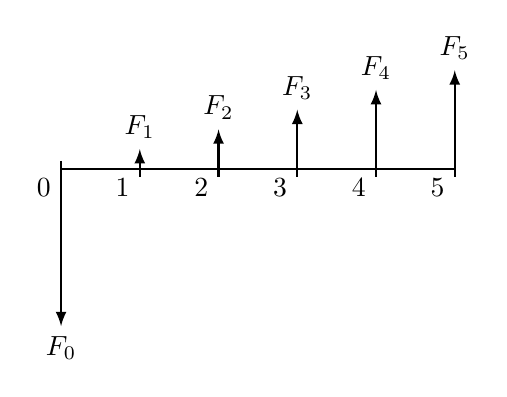
\begin{tikzpicture}[thick]
        \draw (0,0) -- (5,0);
        \foreach \Y [count=\X starting from 0] in {-2, 0.25, 0.5, 0.75, 1, 1.25}
        {\draw[-latex] (\X,0) node[below left]{\X} (\X,{-0.1*sign(\Y)}) -- (\X,\Y)
        node[anchor={sign(\Y)*(-90)}]{$F_{\X}$};}
    \end{tikzpicture}
}
\subsection*{AW of a Perpetual Investment}
\begin{enumerate}
    \item If an investment has no finite cycle, it is called a perpetual investment.
    \item If "P"
\end{enumerate}




\end{document}

